\documentclass{article}
\usepackage[utf8]{inputenc}
\usepackage[right=2cm,left=3cm,top=2cm,headsep=0.5cm,footskip=0.5cm]{geometry}

\title{The Impossible  Early Galaxy Problem}
\author{Santiago Arranz Sanz }
\date{June 2019}

\usepackage{natbib}
\usepackage{graphicx}
\usepackage{latexsym}
\usepackage{eufrak}
\usepackage{dsfont}
\usepackage{hyperref}
\usepackage{enumerate} 
\usepackage{lscape}
\usepackage{titlesec}
\usepackage{fancyhdr}
\usepackage{color}


\newtheorem{teo}{\underline{Teorema}}
\newtheorem{defi}{\underline{Definici\'on}}
\newtheorem{propo}{\underline{Proposici\'on}}
\newtheorem{ejem}{\underline{Ejemplo}}[section]
\newtheorem{prob}{\underline{Problema}}
\newtheorem{lema}{\underline{Lema}}
\newtheorem{obs}{\underline{Observaci\'on}}
\newtheorem{ide}{\underline{Idea}}

\begin{document}

\maketitle

\section*{Introduccion}

Después de leer varios artículos en los que trata dicho problema y derivados he llegado a la conclusión que el problema base es la discordancia del modelo actual de fusión jerárquica con la falta de observación de galaxias transitorias entre los halos iniciales y las galaxias más masivas en los redshift $z\sim 4-6$. Veamos algunos resumenes de los artículos principales.

\section*{The Impossible Early Galaxy Problem}
\citep{steinhardt2016impossibly} Según el paradigma actual de la fusión jerárquica de galaxias en el modelo cosmológico estandar, en torno a los redshift $z\sim 4-6$ ha de existir la transición de las galaxias más masivas desde los halos iniciales que acretan masa a las últimas fases de evolución bariónica vista en las galaxias con formación estelar y \textit{quasars}. Sin embargo, ninguna evidencia ha sido encontrada en muchos estudios a alto redshift como el CFHTLS, CANDELS y el SPLASH, los primeros estudios para probar la masa alta final en estos redshift. Considerando que el ratio masa estelar- masa halo (SMHMR) estimado a bajo redshift permaneciera constante en $z\sim 6-8$, CANDELS y SPLASH darían mayores ordenes de magnitud de número de halos de masa $M\sim 10^{12-13}M_\odot$ que los que se podrían haber formado a esos redshift, esto se conoce como el problema de la galaxia masiva temprana imposible. En el artículo de \cite{steinhardt2016impossibly} consideran los posibles errores sistemáticos que puedan explicar esta contradicción de teoría y observaciones en los modelos de síntesis estelar usados para estimar los parámetros físicos  y en los escenarios posibles de formación galáctica. Es posible que las incertidumbres desconocidas reduzcan la disparidad entre observaciones y simulaciones de CMD tomando una visión conservadora de las observaciones,aun así existirían tensiones considerables con la teoría.\\

Existe un consenso bastante amplio en la distribución de masa y redshift de los halos producidos en el colapso inicial de las pequeñas fluctuaciones de densidad en el universo temprano y el modelo de fusión jerárquico. Para la cosmología estándar la función de masa es sencilla de calcular. Este consenso se basa en la idea de la rápida evolución en la densidad de halos masivos en $z>4$ que deberían ser observacionalmente evidente en las funciones de masa y luminosidad galácticas. Hasta hace poco el catálogo de galaxias a redshift $z>6$ era limitado y sesgado a las galaxias más brillantes, galaxias individuales masivas y \textit{quasars}. Sin embargo con los nuevos estudios como el CANDELS o el SPLASH se ha podido probar la función de luminosidad y de masa para galaxias en el rango de $z\sim 4-8$, lo que nos permite calcular la función de masa del halo correspondiente a dicho rango.\\

Trabajos como el de \cite{finkelstein2015increasing} muestra las tensiones ocasionadas en $z>4$ entre la evolución esperada de la función de masa del halo y las funciones de luminosidad y de masa de las galaxias.\footnote{El resumen de dicho trabajo lo podemos encontrar en \cite{arranz2015finkelstein}} \\

\section*{Galaxias tempranas y sus halos}
Como hemos visto en el trabajo de \cite{finkelstein2015increasing} la teoría espera una rápida evolución en las galaxias entre los redshift de $z=4-7$, sin embargo las observaciones no avalarón dichas prediccionas en su trabajo. En el trabajo de \cite{steinhardt2016impossibly} pretende extender y actualizar los resultados de trabajos como el de \cite{finkelstein2015increasing} basándose en los datos de CANDELS y SPLASH. La ventaja de tomar redshift altos como los del estudio de $z=4-8$ es que tenemos un tiempo cósmico más pequeños (0.9 Gyr \citep{steinhardt2016impossibly}) en un mayor número de redshift, lo que debiese permitir ver una evolución mas detallada que en redshift bajos. Por otro lado los métodos de estimación de las masas de los halos son menos abundantes por lo que el trabajo de \cite{steinhardt2016impossibly} trabaja básicamente con tres tipos de estimaciones.
\begin{enumerate}
\item El primero de ellos se base en la clusterización \citep{hildebrandt2009cars} el cual estima la masa del halo según la distribución espacial de las galaxias. La ventaja de este método es que no hay que asumir ninguna propiedad física de las galaxias, pero sí es necesario escoger un modelo de materia oscura para las simulaciones.
\item Un segundo método es el presentado y desarrollado en el artículo de \cite{finkelstein2015increasing}, el cual se basa en la curva de luminosidad UV \footnote{Hay que recordar que podría ser incorrecta ya que en el artículo de se asumio la existencia de galaxias solo visibles en submilimétricas \citep{wang2019dominant}.} y en la función de masa calculada a través de simulaciones, relacionando ambas por el principio de que el halo más masivo a de albergar la galaxia más masiva y viceversa.
\item El último método es asumir un ratio entre luminosidad/masa estelar y materia oscura. El ratio asumido es el redshift más bajos donde las estimaciones de materia oscura son más factibles por los métodos de agrupación. El ratio usado para el enlace entre masa estelar y de halo es  $M_h/M_\star \sim 70 $.
\end{enumerate}

\textcolor{red}{Sobre el primer método no puedo decir mucho de momento ya que no he leido el paper de \cite{hildebrandt2009cars} donde desarrollan el método, pero al igual que en el último método depende de un modelo de materia oscura lo cual podría ser una variable a tener en cuenta para que los resultados cuadren con las observaciones. Sobre el segundo método ya se ha discutido los posibles fallos en \cite{arranz2015finkelstein} que puede tener sobre todo a raiz del descubrimiento de \cite{wang2019dominant}. Por último considera un ratio igual a redshift más bajos lo cual no tendría porque ser cierto si las propiedades de galaxias y halos evolucionan con el tiempo, lo que podría demostrar el artículo de \cite{wang2019dominant} contradiciendo las suposiciones realizadas en \cite{finkelstein2015increasing}. Todos estos puntos débiles pueden ser clave fundamental para poner en duda dichos resultados.}\\

\begin{figure}[h]
\begin{center}
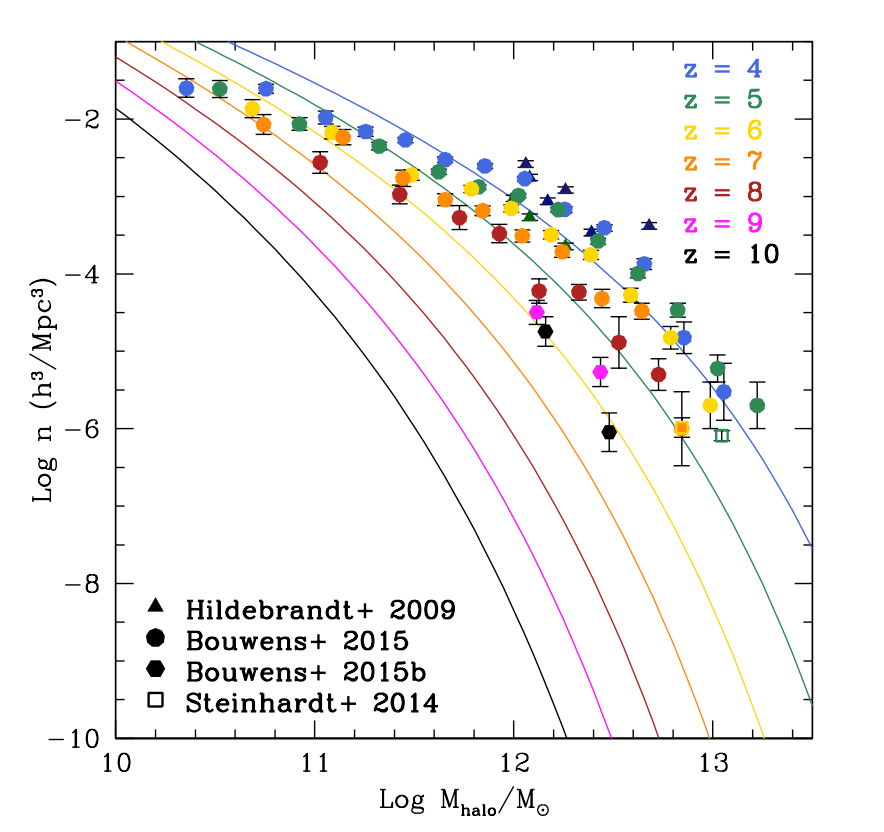
\includegraphics[scale=0.55]{Figuras/steindhart_fig1.png}
\caption{\label{fig:steindhart_fig1} Imagen que representa las estimaciones teoricas del número de densidad de halos en función de su masa versus las obtenidas de las observaciones estudiadas en \cite{steinhardt2016impossibly}}
\end{center}
\end{figure}

Las estimaciones teóricas de la función de masa de los halos para los diferentes redshift han sido sacadas de la herramienta \cite{murray2013hmfcalc} la cual esta basada en el trabajo \cite{sheth2001ellipsoidal}. Las discrepancias que se pueden observar en la \textbf{Figura \ref{fig:steindhart_fig1}} son muy visibles, en especial se encuentran la función de masa del halo de las observaciones tienen un mayor número de densidad de halos masivos con respecto a los predichos por la teoría. Una posible explicación es que el ratio $M_h/L_{UV}$ en galaxias masivas decrece bruscamente en $z>4$, tendiendo a sobrestimar la masa de halos de las galaxias de alto redshift. Si esto fuera así se podría esperar que esta rápida evolución tuviera que ser evidente en otras propiedades medibles de la población de galaxias. En el siguiente punto del artículo de \cite{steinhardt2016impossibly} trata esta posibilidad sin encontrar ninguna evidencia de dicha evolución del ratio de masa halo y luminosidad. \textcolor{red}{Esta posibilidad solo explicaría las medidas basadas en luminosidad, quedando fuera quizás el primer método de clusterización. Por otro lado, la evolución drástica en luminosidad podría hacer que no se viesen todas las galaxias del halo \citep{wang2019dominant} por lo que afectaría a las medidas basadas en clusterización del primer método}

\section*{Aspecto normal de las galaxias en alto redshift}
Se ha denominado como \textit{Impossible early galaxy problem} a la brusca discrepancia de las estimaciones de la función de masa de halo entre las observaciones y teorias. Esta discrepancia podría explicarse si no asumimos que el comportamiento de las galaxias en redshift altos es similar a las de bajo redshift, esto podría dar una solución sencilla al problema. Si encontráramos diferencias entre las galaxias de alto y bajo redshift, que permitieran suponer que no es correcto adoptar plantillas de ajustes del SED y relaciones de escala tomadas en redshift bajos en galaxias de altos redshift, podríamos poner en cuestión las estimaciones observacionales que relajarían la tensión con la teoría. \textcolor{red}{Este creo que es el principal punto, veamos como encaja las nuevas observaciones de \cite{wang2019dominant} en este marco y si son relevantes en este punto}\\

En las últimas décadas se ha observado que muchos procesos, incluyendo la formación estelar, ocurre mas temprano en las galaxias más masiva que en las menos masivas. La evolución temprana de las galaxias masivas y con formación estelar es también soportada por la observación de galaxias masivas y pasivas en redshift $z\sim 2-4$. Además, los ratios de FeII/MgII en quasars de alto redhistf y las edades derivadas de los ajustes de los SED sugieren que las galaxias masivas y tempranas necesitan formas sus estrellas más rápidamente.\\

Por otro lado, la teoría $\Lambda$CDM necesita que los halos más masivos generalmente acreten más tarde la matería que sus compañeros menos masivos. Por tanto, reconciliar la teoría y las observaciones requiere que las galaxias más masivas puedan evolucionar más rápido que las menos masivas. Ya que el tiempo dinámico incrementa con la masa, una evolución rápida en redshift altos podría necesitar de que la física de los procesos bariónicos que dominan la formación estelar sea modificada con respecto a redshift más bajos. Por tanto en el modelo se debería predecir que en el intervalo de redshift $z\sim 4-8$ una rápida transición entre los procesos de acreción de los halos y el rápido crecimiento de las poblaciones estelares. \\

\textcolor{red}{Observamos otra discrepancia entre teoría y observación, si la acreción de masa en los halos masivos tiene un mayor tiempo de duración que en los más pequeños en estos últimos el gas se debería de enfriar antes y deberían de poder formar estrellas con más rapidez. Sin embargo, se observa que las galaxias más masivas (asociadas a los halos más masivos) forman sus estrellas más rápido que los menos masivos (asociados a los menos masivos). Al igual que ocurre en el análisis de \cite{finkelstein2015increasing} \citep{arranz2015finkelstein} entra en cuestión la suposición de que las galaxias más masivas se encuentran en los halos más masivos, quizás las dinámicas en la acrección de masa en los halos masivos impidan la formación de galaxiás masivas, produciendo una mayor cantidad de galaxias menos masivas quedando las galaxias masivas en halos menos masivos. Esto debería de indicar una relación masa halo y masa estelar menor de lo esperado lo cual podría ser estudiado con RAMSES. Por otro lado, tomando por buena esta suposición se deduce que los procesos de la física barionica implicados en la formación estelar han de ser distintos en redshift altos, por ejemplo los tiempos de enfriamiento, lo cual debería de dejar una señal entre las galaxias de redshift 4 y 8.}\\

\subsection*{Similitudes de la relación SFR-Masa estelar entre galaxias de alto y bajo redshift.}

Hasta la fecha, CANDELS y SPLASH no han encontrado desviaciones aparentes de las propiedades derivadas en redshift bajos. En cambio, encuentran que la tendencia a que más y más galaxias masivas evolucionen antes continúa hasta $z \sim 6 - 8$. En particular, a $0< z <4$ se ha demostrado que las galaxias formadoras de estrellas se encuentran en una "secuencia principal" \citep{Renzini_2015}, con una estrecha correlación entre la masa estelar existente y su tasa de formación de estrellas. Un análisis de más de dos docenas de estudios de galaxias formadoras de estrellas utilizando diferentes técnicas para la selección, para medir la masa estelar y para medir la tasa de formación de estrellas muestra un fuerte acuerdo en la evolución de la pendiente y el desplazamiento al rojo.
Las primeras galaxias de alto desplazamiento al rojo se encuentran en la extrapolación de esta secuencia principal a $z \sim 6-7$.\\

La secuencia principal de formación estelar está bien medida para objetos de menor masa en $z\sim 5-6$ entre SPLASH y CANDELS. Donde hay masas estelares disponibles, las galaxias tempranas más masivas se encuentran directamente en la extrapolación de gran masa de esta secuencia principal. Debido a que la masa estelar y las tasas de formación de estrellas se miden usando diferentes longitudes de onda, los errores sistemáticos del ajuste incorrecto de la plantilla producirían cantidades inferidas incorrectas de diferentes maneras, y probablemente producirían una población inconsistente con la secuencia principal. Del mismo modo, los problemas de desmembramiento arbitrario producirían valores atípicos ubicados en algún lugar arbitrario y, por lo tanto, probablemente fuera de esta secuencia principal. \textcolor{red}{Diferentes medidas en diferentes longitudes de ondas nos llevan al mismo resultado, en el caso de haber errores sistemáticos cada una de esas medidas tendrían un error y por tanto los resultados serían muy aleatorios. Entiendo que es ese el argumento dado.} \\

La evolución de desplazamiento al rojo de la secuencia principal de formación estelar también se entiende bien en $0<z<4$, y la secuencia principal de formación de estrellas $4<z<6$ observada tiene las propiedades producidas extrapolando esa dependencia del tiempo. El aumento de la masa hacia el alto desplazamiento al rojo de las N galaxias formadoras de estrellas más masivas (un componente de lo que se ha denominado el problema de ``\textit{downsizing}''\footnote{El problema de \textit{downsizing} trata que los moedelos actuales de fomración galáctica predicen que las primeras galaxias formadas son las de baja masa mientras que en las observaciones se ven que las galaxías con poblaciones mas antiguas de estrellas son las más masivas. Se ve ademas en redshift altos que las formadoras de estrellas son las galaxias masivas cuando en teoría deberían de ser las menos masivas.}) también está bien medido, y las galaxias formadoras de estrellas más masivas en $z\sim6$ se encuentran en la extrapolación de la dependencia del tiempo de mejor ajuste en $0<z<4$ (\textbf{Figura \ref{fig:steindhart_fig2}}). \textcolor{red}{La \textbf{Figura \ref{fig:steindhart_fig2}} Parecer mostrar muy claramente dicha relación, se ve una relación lineal muy estrecha aunque pudiera ser por selección de datos.} \\

\begin{figure}[t]
\begin{center}
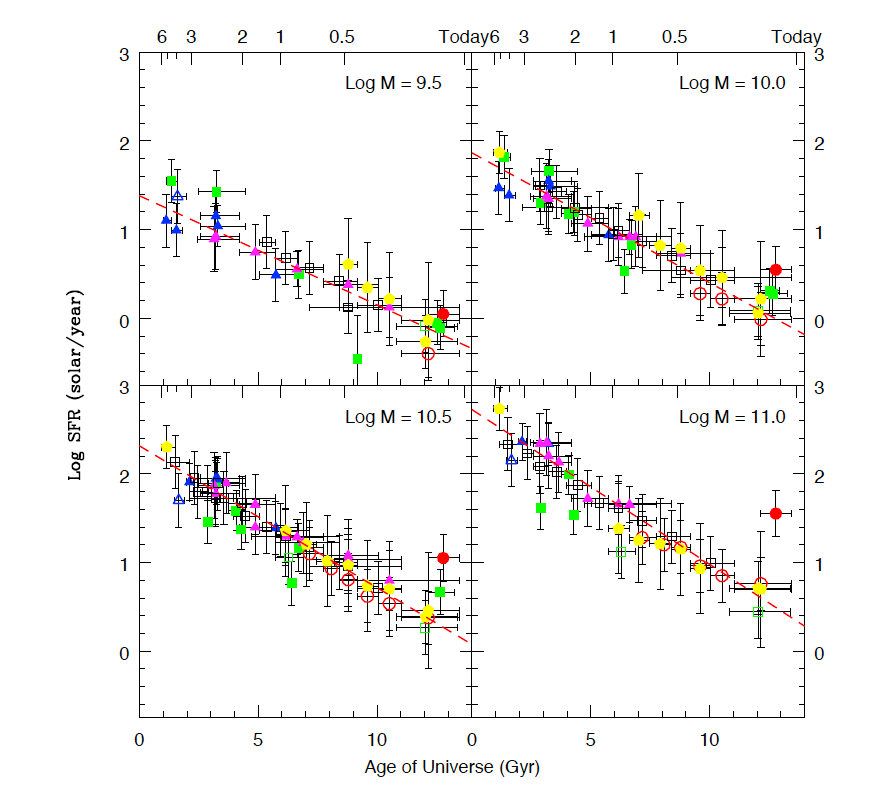
\includegraphics[scale=0.55]{Figuras/steindhart_fig2}
\caption{\label{fig:steindhart_fig2} 96 mediciones de 32 estudios de la secuencia principal de formación de estrellas 4 para $M_\star$ fijo $= 10^{10.5}M_\odot$ a $0 <z <6$, ajustado para ubicarse en un conjunto común de calibraciones siguiendo la prescripción derivada por \cite{speagle2014highly} utilizando 25 de estos estudios. Las barras horizontales indican el rango de redshift que abarca cada observación en particular, mientras que los errores verticales son la verdadera dispersión sobre cada observación de la secuencia principal \citep{speagle2014highly}. Aunque estos estudios utilizan muchos métodos diferentes para determinar la SFR y la masa estelar (azul = UV, púrpura = UV + IR, rojo = IR, verde = líneas de emisión, amarillo = ajuste SED, negro = radio), todos muestran un buen acuerdo con  la evolución lineal de mejor ajuste (log) determinada en $0 <z <4$ (línea de puntos), y las mediciones del redshift más altas son consistentes con la extrapolación de ese ajuste a $z\sim 6$. Por lo tanto, parece probable que las técnicas para estimar estelares las masas y las tasas de formación estelar no se han vuelto catastróficamente incorrectas en $z\sim 6$.}
\end{center}
\end{figure}

En algún momento, las plantillas estelares derivadas de un desplazamiento hacia el rojo bajo dejarán de ser válidas, pero esto aún no se ha observado. Podría esperarse que esto ocurra solo cuando la física de la formación estelar haya cambiado, tal vez debido a unas metalicidades muy bajas que producen un IMF muy pesado e incluso estrellas de la Población III \footnote{¿Sobre redshift $z\sim 20$?}. Si es así, las plantillas pueden seguir siendo válidas muy por encima de $z\sim 6-8$. Como mínimo, parece claro que no se han vuelto catastróficamente incorrectos en el rango de desplazamiento al rojo donde se han medido imposiblemente las primeras galaxias.\\

\textcolor{red}{El \textit{downsizing} parece otra cara del mismo problema. En \citep{arranz2015finkelstein} se vió el problema de que la densidad de galaxias masivas luminosas parecía mantenerse en el rango de redshift $4<z<7$ mientras que el número de densidad de galaxias bajaba con el aumento del redshift. Parecía que las galaxias luminosas se mantienen siendo estás las primeras en formar estrellas, al contrario de lo que predice la teoría y las simulaciones. La pregunta es si falla la teoría, las observaciones o ambas opciones.}

\subsubsection*{Relación Galaxia - Quasar}

Al igual que ocurre con el número de galaxias de formación estelar, la presencia de quasares plantea un problema similar en redshift altos, ya que parecen ser más lusminosos y con agujers negros más masivos con un mayor redshift. Este problema se ha conocido como ``\textit{impossibly early black hole}'' de manera análoga al problema que estamos estudiando.\\

Una parametrización de la similitud entre la evolución del redshift de los cuásares y las galaxias formadoras de estrellas es observar que la relación de $M_\star$ para la mayoría de las galaxias formadoras de estrellas masivas con respecto a $M_{BH}$ para los cuásares más masivos se observa que es aproximadamente $30:1$ en todo redshift fijo. Las galaxias $log M_\star / M_\odot\sim11.2$ en $z\sim 6$ en SPLASH tienen una relación similar con los primeros cuásares masivos, como el quasar $log M_{BH} / M_\odot\sim 10.08$  en $z = 6.4$ estudiado en \cite{wu2015ultraluminous}. Porque las estimaciones de masa del agujero negro virial tienen incertidumbres sistemáticas muy diferentes a las estimaciones de masa estelar, esta relación que sigue siendo una evidencia adicional de que las propiedades inferidas para las galaxias imposiblemente tempranas son probablemente razonables.\\

Se espera que a un redshift lo sufucientemente grande varias de estas relaciones de escala se vengan a bajo, pero aún no se ha podido observar. El punto clave es que la población observada de galaxias formadoras de estrellas  en redshift altos  sigue la evolución esperada hacia el redshift determinada observacionalmente a partir de muchos estudios de redshift más bajo. Incluso los objetos más masivos y de redhift más altos se encuentran y analizan utilizando las mismas técnicas estándar que se ha verificado que tienen éxito en el redshift más bajo,siendo extraños únicamente por la discrepancia entre la observación y el $\Lambda$CMD, no por los datos.\\

\textcolor{red}{Parece haber una reticencia en el artículo en admitir la posibilidad de que las técnicas de análisis que se aplican en redshift bajos no sean válidas en redshift altos. No me queda del todo claro como se mide la similitud de las propiedades de galaxias en bajo y alto redshift, tampoco como se realiza la extrapolación de las características de bajo redshift a alto redshift que tanto se citan. Por otro lado la \textbf{Figura \ref{fig:steindhart_fig2}} parece mostrar perfectamente la relación mostrada en la secuencia principal, donde el slope parece mantenerse (creciendo con el redshift) y aumentar el punto de intersección con una mayor masa estelar.}

\subsection*{Función de luminosidad para determinar la masa del Halo.}
Las funciones de luminosidad UV son una de las más baratas y más robustas observaciones para obtener en redshift altos y se pueden convertir en masas de halo suponiendo una relación de masa a luz de halo. De hecho, la mayoría de los datos de alto redshift que se muestran en la \textbf{Figura \ref{fig:steindhart_fig1}} y todos aquellos en $z> 6$ se derivan de las funciones de luminosidad UV monocromática , las únicas observaciones disponibles. La principal ventaja de esta técnica sobre las funciones de masa es que coloca la mayor parte de la incertidumbre potencialmente grande en la relación masa-luz del halo, que se puede parametrizar en un solo modelo donde se puede analizar con mayor claridad. En contraste, las funciones de masa colocan gran parte de la incertidumbre en los detalles del conjunto diverso de modelos de distribución de energía espectral que se ajustan a cada galaxia individual donde pueden ser difíciles de entender.
\newpage
\bibliographystyle{plainnat}
\bibliography{references}

\newpage
\appendix
\section*{Planteamientos iniciales de cada día de trabajo}
Notas que pretenden estructurar el trabajo día a día
\subsection*{Agosto 2019}
A falta de terminar de analizar el paper de \cite{finkelstein2015increasing} y de hacer una lista de las dudas surgidas y propuestas a dar ya he leido el artículo de \cite{wang2019dominant} sobre las galaxias a redshift $z>3$ descubiertas por ALMA las cuales parecen ser abundantes y masivas y no detectables por el HST. Esto tumbaría la susposición de \cite{finkelstein2015increasing} de la no existencia o poca abundancia de las galaxías sub-milimétricas lo que modificaría la función de luminosidad y por tanto la relación de masa halo - masa estelar ya que en el paper de \cite{finkelstein2015increasing} se basa principalmente en ella. La propuesta de lo que quiero hacer hoy es lo siguiente:
\begin{enumerate}
\item Terminar el análisis de \cite{finkelstein2015increasing}. $\surd$
\item Como encaja las nuevas observaciones de \cite{wang2019dominant} en el paper de \cite{finkelstein2015increasing} $\surd$
\item Plantear como incluir los planteamientos de \cite{wang2019dominant}: 
\begin{enumerate}[i.]
\item Replantear la función de luminosidad de \cite{finkelstein2015increasing}.
\item Como encaja en el modelo jerárquico \citep{bower2006breaking}.
\item Las simulaciones de RAMSES nos pueden dar un orden distinto a la masa de los halos que encajen de una manera distinta de con la función de luminosidad. 
\end{enumerate}
\end{enumerate}

\subsection*{Septiembre 2019}
\subsubsection*{Semana 2: 9-15}
El artículo de \cite{wang2019dominant} parece indicar que algunas de las suposiciones en las que se basan los métodos de cálculo de las masa de halo están equivocados, por lo que el escenario más factible para la resolución del problema de \cite{steinhardt2016impossibly} sea el error observacional. Las tareas para esta semana son las siguientes:
\begin{enumerate}
\item Terminar el análisis de \cite{steinhardt2016impossibly}.
\item Leer el artículo de \cite{sheth2001ellipsoidal} y \cite{murray2013hmfcalc} que trata las estimaciones teóricas usadas para el cálculo de la función de masa de halo. Empezar con el resumen de \cite{sheth2001ellipsoidal}.
\item Terminar el punto 3 de agosto.
\item Escribir a Santi con los avances el domingo día 15 y plantear con él una reunión.
\end{enumerate}
\end{document}
